% !TEX root = ../tradeoff.tex

%------------------------------------------------------------------------------------------------------------%
\section{Numerical Simulations\label{S:numerics}}
%------------------------------------------------------------------------------------------------------------%


We numerically simulated the reconstruction of a quantum state given Pauli measurements and the estimators from Eqs.~(\ref{eqn-ds}) and (\ref{eqn-lasso}). Here we compare these estimates to those obtained from a standard maximum likelihood estimate (MLE) as a benchmark. 

As mentioned previously, all of our estimators have the advantage that they are convex functions with convex constraints, so the powerful methods of convex programming~\cite{Boyd2004} guarantee that the exact solution can be found efficiently and certified. We take full advantage of this certifiability and do simulations which can be certified by interior-point algorithms. This way we can separate out the performance of the estimators themselves from the (sometimes heuristic) methods used to compute them on very large scale instances. 

For our estimators, we will explicitly enforce the positivity condition. That is, we will simulate the following slight modifications of Eqs.~(\ref{eqn-ds}) and (\ref{eqn-lasso}) given by
\begin{equation}\label{E:new-ds}
	\hat{\rho}_\ds' = \arg\min_{X\succeq0}\, \Tr X \st \norm{\calA^*(\calA(X)-y)} \leq \lambda\,,
\end{equation}
and
\begin{equation}\label{E:new-lasso}
	\hat{\rho}_\lasso' = \arg\min_{X\succeq0}\, \tfrac{1}{2} \norm{\calA(X)-y}_2^2 + \mu \Tr X \,.
\end{equation}
Moreover, whenever the trace of the resulting estimate is is less than one, we renormalize the state, $\hat\rho \mapsfrom \hat\rho/\Tr(\hat\rho)$. 

%------------------------------------------------------------------------------------------------------------%
\subsection{Setting the Estimator Parameters \texorpdfstring{$\lambda$}{lambda} and \texorpdfstring{$\mu$}{mu}}
%------------------------------------------------------------------------------------------------------------%


From Thm.~\ref{thm-errorbound} we know roughly how we should choose the free parameters $\lambda$ and $\mu$, modulo the unknown constants $C_i$, for which we will have to make an empirical guess. We guess that the log factor is an artifact of the analysis, and that the state is nearly pure. Then we could choose $\lambda \sim \mu \sim d/\sqrt{t}$. For the matrix Dantzig selector of \Eref{E:new-ds}, we specifically  chose $\lambda = 
3 d/\sqrt{t}$ for our simulations. However, this did not lead to very good performance for the matrix Lasso of \Eref{E:new-lasso} when $m$ was large. We chose instead $\mu = 4 m/\sqrt{t}$, which agrees with $\lambda$ when $m \sim d$, as it can be for nearly pure states. 

We stress that very little effort was made to optimize these choices for the parameters. We simply picked a few integer values for the constants in front (namely $2,\dots,5$), and chose the constant that worked best upon a casual inspection of a few data points. We leave open the problem of determining what the optimal choices are for $\lambda$ and $\mu$. 


%------------------------------------------------------------------------------------------------------------%
\subsection{Time Needed to Switch Measurement Settings}
%------------------------------------------------------------------------------------------------------------%


Real measurements take time. In a laboratory setting, time is a precious commodity for a possibly non-obvious reason. An underlying assumption in the way we typically formulate tomography is that the unknown state $\rho$ can be prepared identically many times. However, the parameters governing the experiment often drift over a certain timescale, and this means that beyond this characteristic time, it is no longer appropriate to describe the measured ensemble by the symmetric product state $\rho^{\otimes t}$.  

To account for this characteristic timescale, we introduce the following simple model.  We assume that the entire experiment takes place in a fixed amount of time $T$.  In a real experiment, this is the timescale beyond which we cannot confidently prepare the same state $\rho$, or it is the amount of time it takes for the student in the lab to graduate, or for the grant funding to run out, whichever comes first.  Within this time limit, we can either change the measurement \emph{settings}, or we can take more \emph{samples}.  We assume that there is a unit cost to taking a single measurement, but that switching to a different measurement configuration takes an amount of time $c$.

At the one extreme, the switching cost $c$ to change measurement settings could be quite large, so that it is only barely possible to conduct enough independent measurements that tomography is possible within the allotted time $T$.  In this case, we expect that compressed tomography will outperform standard methods, since these methods have not been optimized for the case of incomplete data.  At the other extreme, the switching cost $c$ could be set to $0$ (or some other small value), in which case we are only accounting for the cost of sampling.  Here it is not clear which method is better, for the following reason.  Although the standard methods are able to take a sufficient amount of data in this case, each observable will attain comparatively little precision relative to the fewer observables measured with higher precision in the case of compressed tomography for the same fixed amount of time $T$. One of our goals is to investigate if there are any tradeoffs in this simple model. 

For the relative cost $c$ between switching measurement settings and taking one sample, we use $c = 20$, a number inspired by the current ion trap experiments done by the Blatt group in Innsbruck. However, we note that the conclusions don't seem to be very sensitive to this choice, as long as we don't do something outrageous like $c > t$, which would preclude measuring more than even one observable. 


%------------------------------------------------------------------------------------------------------------%
\subsection{Other Simulation Parameters\label{S:params}}
%------------------------------------------------------------------------------------------------------------%


We consider the following ensembles of quantum states. We initially choose $n=5$ qubit states from the invariant Haar measure on $\C^{2^n}$. 
Then we add noise to the state by applying independent and identical depolarizing channels to each of the $n$ qubits. Recall that the depolarizing channel with strength $\gamma$ acts on a single qubit as
\begin{align}
	\mathcal{D}_\gamma(\rho) = \gamma \frac{\one}{2} + (1-\gamma) \rho \,,
\end{align}
that is, with probability $\gamma$ the qubit is replaced by a maximally mixed state and otherwise it is left alone. Our simulations assume very weak decoherence, and we use $\gamma = 0.01$.

We use two measures to quantify the quality of a state reconstruction $\hat\rho$ relative to the underlying true state $\rho$, namely the (squared) fidelity $\lVert \sqrt{\hat\rho}\sqrt{\rho}\rVert^2_\tr$ and the trace distance $\frac{1}{2} \norm{\rho - \hat\rho}_\tr$.

We used the interior-point solver SeDuMi~\cite{Sturm1999} to do the optimizations in Eqs.~(\ref{E:new-ds}) and (\ref{E:new-lasso}). Although these algorithms are not suitable for large numbers of qubits, they produce very accurate solutions, which allows a more reliable comparison between the different estimators.  The data and the code used to generate the data for these plots can be found with the source code for the arXiv version of this paper. For larger numbers of qubits, one may instead use specialized algorithms such as SVT, TFOCS, or FPCA to solve these convex programs~\cite{Cai2010,Becker2010,Ma2011}; however, the quality of the solutions depends somewhat on the algorithm, and it is an open problem to explore this in more detail.

For the MLE, we used the iterative algorithm of Ref.~\cite{Rehacek2001}, which has previously been used in e.g.\ Ref.~\cite{Molina-Terriza2004}. This method converged on every example we tried, so we did not have to use the more sophisticated ``diluted'' method of Ref.~\cite{Rehacek2007} that guarantees convergence. 

For the purposes of our simulations, we sampled our Pauli operators \emph{without} replacement. 


%------------------------------------------------------------------------------------------------------------%
\subsection{Results and Analysis}
%------------------------------------------------------------------------------------------------------------%


\begin{figure}[t!]
\centering
\begin{tabular}{c}
a)\hspace{-10pt} 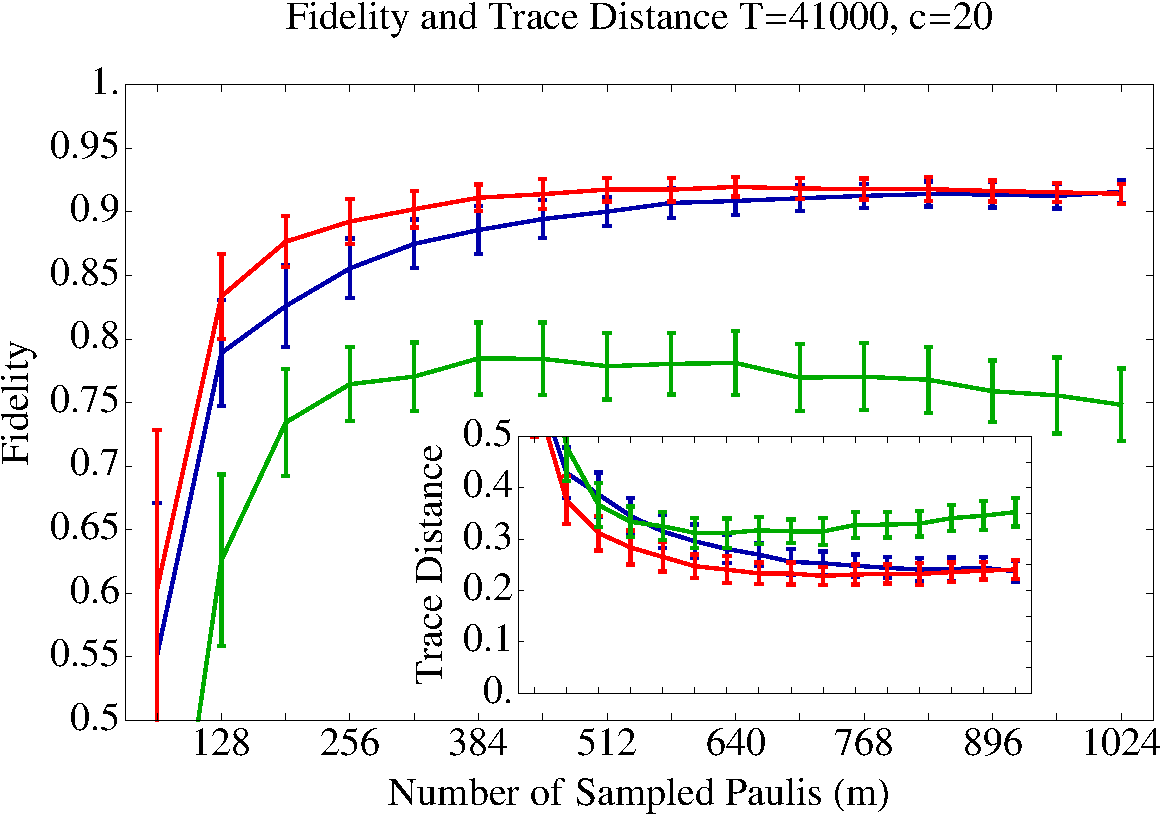
\includegraphics[scale=.42]{figures/41} \vspace{5pt}\\
b)\hspace{-10pt} 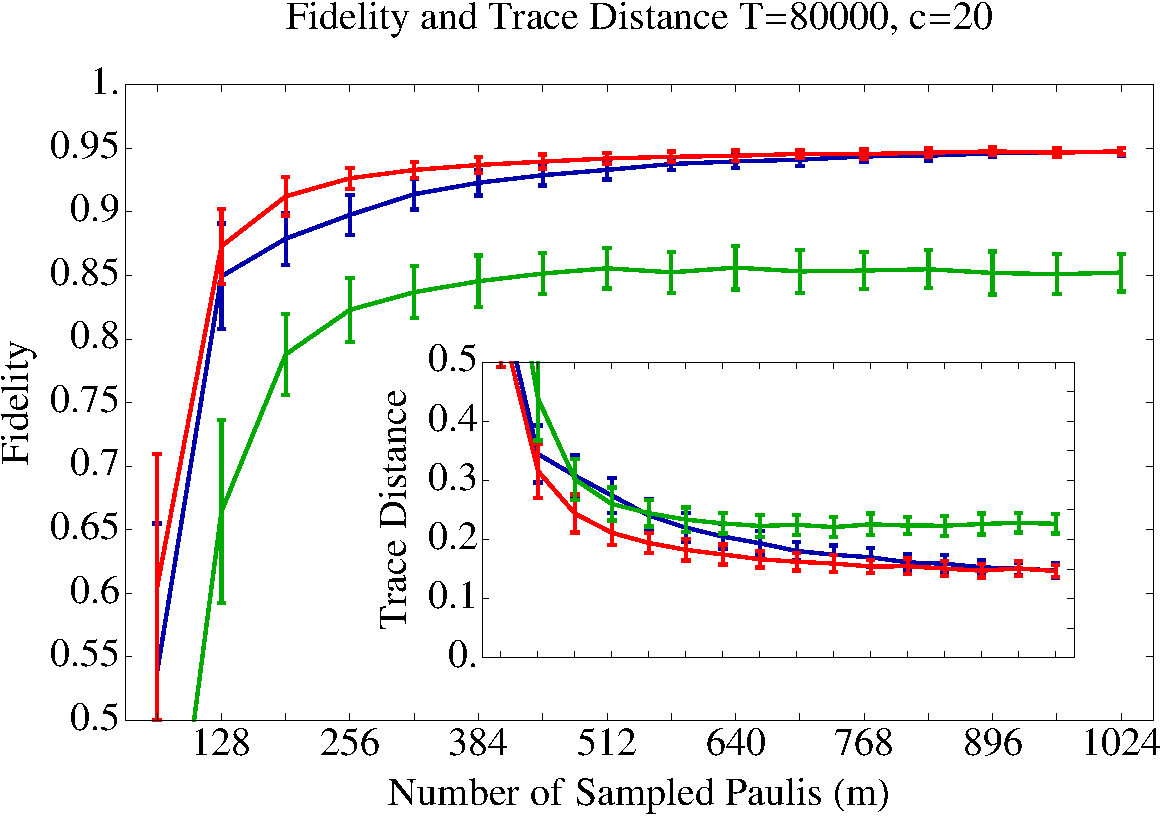
\includegraphics[scale=.42]{figures/80}  \vspace{5pt}\\
c)\hspace{-10pt} 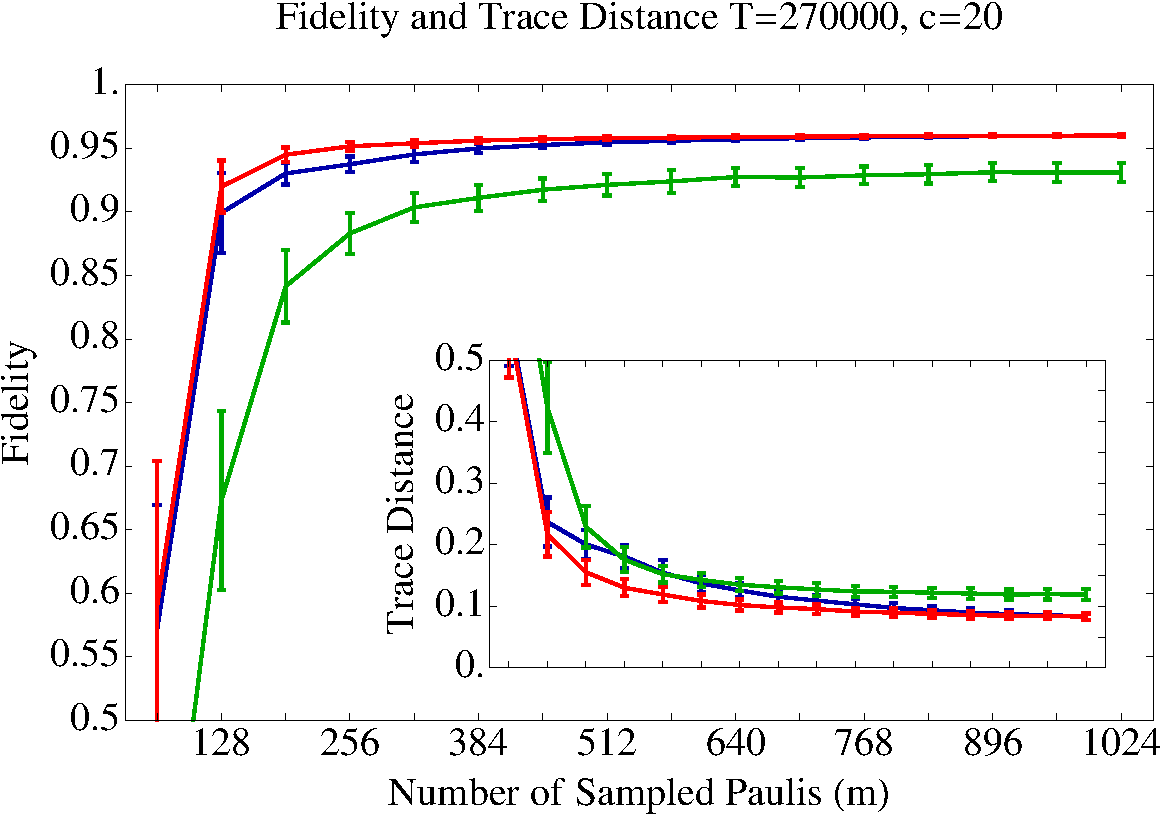
\includegraphics[scale=.42]{figures/270}
\end{tabular}
\begin{caption}{\label{F:numerics}Fidelity and trace distance (inset) as a function of $m$, the number of sampled Paulis. Plots a), b) and c) are for a total measurement time of $T=41$k, $80$k, and $270$k respectively, in units where the cost to measure a single copy is one unit of time, and the cost to switch measurement settings is $c=20$ units. The three estimators plotted are the matrix Dantzig selector (\Eref{E:new-ds}, blue), the matrix Lasso (\Eref{E:new-lasso}, red), and a standard MLE (green). Each bar shows the mean and standard deviation from 120 Haar-random 5-qubit states with 1\% local depolarizing noise. Our estimators consistently outperform MLE, even after optimizing the MLE over $m$. See the main text for more details.\vspace{-5pt}}
\end{caption}
\end{figure}


The data are depicted in Fig.~\ref{F:numerics}. The three subfigures a--c use three different values for the total sampling time $T$ in increasing order. We have plotted both the fidelity and the trace distance (inset) between the recovered solution and the true state. %We note that a simple least squares estimator performed worse than all the others, so we do not include a plot of that here.

Several features are immediately apparent. First, we see that both of the compressed sensing estimators consistently outperform MLE along a wide range of values of $m$, the number of Paulis sampled, even when we choose the optimal value of $m$ just for the MLE. Once $m$ is sufficiently large (but still $m \ll d^2$) \emph{all} of the estimators converge to a reasonably high fidelity estimate. Thus, it is not just the compressed sensing estimators which are capable of reconstructing nearly low rank states with few measurement settings, but rather this seems to be a generic feature of many estimators. However, the compressed sensing estimators seem to be particularly well-suited for the task. 

When the total amount of time $T$ is \emph{very} small (Fig.~\ref{F:numerics}a), then there is a large advantage to using compressed sensing. In this regime, there is barely enough time to make one measurement per setting if we insist on making an informationally complete measurement, so the measurement statistics aren't even Gaussian. Thus, the fluctuations are so large that trying to fit a density operator to these data just leads to poor results because you wind up fitting only noise. While the advantage of compressed sensing is clear in this regime, it is not applicable when we are interested in extremely high-fidelity state reconstructions (namely greater than 95\%). 

As the total amount of time available increases, all of the estimators of course converge to higher fidelity estimates. Interestingly, for the compressed sensing estimators, there seems to be \emph{no tradeoff whatsoever} between the number of measurement settings and the fidelity once $T$ and $m$ are sufficiently large. That is, the curve is completely flat as a function of $m$ above a certain cutoff. This is most notable for the matrix Lasso, which consistently performs at least as well as the matrix Dantzig selector, and often better. These observations are consistent with the bounds proven earlier. 

The flat curve as a function of $m$ is especially interesting, because it suggests that there is no real drawback to using small values of $m$. Smaller values of $m$ are attractive from the computational point of view because the runtime of each reconstruction algorithm scales with $m$. This makes a strong case for adopting these estimators in the future, and at the very least more numerical studies are needed to investigate how well these estimators perform more generally.

We draw the following conclusion from these simulations. The best performance for a fixed value of $T$ is given by the matrix Lasso estimator of Eqs.~(\ref{eqn-lasso}) and (\ref{E:new-lasso}) in the regime where $m$ is nearly as small as possible. Here the fidelity is larger than the other estimators (if only by a small or negligible amount when $T$ is large), but using a small value for $m$ means smaller memory and processing time requirements when doing the state reconstruction. MLE consistently underperforms the compressed sensing estimators, but still seems to ``see'' the low-rank nature of the underlying state and converges to a reasonable estimate even when $m$ is small. 
